\documentclass{article}
\usepackage[utf8]{inputenc}
\usepackage{amsmath, amssymb, multicol, enumerate, tikz}
\usepackage[margin = 0.5in]{geometry}
\pagestyle{empty}
\raggedright
\newcounter{PS}
\begin{document}

Name \makebox[3in]{\hrulefill} \hfill Honors Algebra 2 PSet

\subsubsection*{Equations and Inequalities \hfill \makebox[0.35in]{\hrulefill} / 10}

Solve each of the following. Check your answers.    
\begin{flalign*}
1. \quad    &	14-5x=-41		&
2. \quad    &	2x-7=6+x		&
3. \quad	&   3(x-2)+7 = 2(x+5)	&&\\[2in]
4. \quad	&	2(x-1)+3=x-3(x+1)	&
5. \quad	&	5x-(2x+2)=x+(3x+5)	&
6. \quad	&	5x+9=9(x+1)-4x		&&\\[3in]
7. \quad	&	3(y+2)=7+3y		&
8. \quad	&   \dfrac{x}{3} = \dfrac{x}{2} - 2	&
9. \quad	&   \dfrac{3x}{5}-x=\dfrac{x}{10} - \dfrac{5}{2}	&&\\
\end{flalign*}

\newpage

Name \makebox[3in]{\hrulefill} \hfill Hon. Alg. 2 P-Set    \newline\\ 

Solve each and graph your answers on a number line. 
\begin{flalign*}
10. \quad    &   5x+11<26		        &
11. \quad	&	3x-8 \geq 13	        &
12. \quad	&	-9x \leq 36	            &&\\[2in]
13. \quad	&	4(x+1) + 2 > 3x+6	    &
14. \quad	&	8x-11 \leq 3x-13	    &
15. \quad	&	2x-11 < -3(x+2)	        &&\\[2in]
16. \quad	&	4(3x-2)-3x < 3(1+3x)-7	&
17. \quad	&	3x \leq 3(x-2)			&
18. \quad	&	1-\dfrac{x}{2} > 4		&&\\[1.5in]
\end{flalign*}

\subsection*{Challenge Problems}

Solve each of the following for the variable indicated.
\begin{flalign*}
19. \quad   &   C = \frac{5}{9}\left(F - 32\right) \text{  for }F  &
20. \quad   &   m = \dfrac{x+y+z}{3} \text{  for }y &
21. \quad   &   A = P(1 + rt) \text{ for t} &&\\
\end{flalign*}

\newpage

\subsection*{Equations and Inequalities Answers}

\subsection*{Equations}
\begin{flalign*}
1. \quad    &   x = 11      &
2. \quad    &   x = 13      &
3. \quad    &   x = 9       &&\\
4. \quad    &   x = -1      &
5. \quad    &   x = -7      &
6. \quad    &   \text{All real numbers } (\mathbb{R})    &&\\
7. \quad    &   \text{No Solution } (\varnothing)   &
8. \quad    &   x = 12      &
9. \quad    &   x = 5       &&\\
\end{flalign*}

\subsection*{Inequalities}  
\vspace{11pt}
\begin{tabular}{p{0.3\textwidth}p{0.3\textwidth}p{0.3\textwidth}}
10. $x < 3$ &   11. $x \geq 7$ &   12. $x \geq 4$  \\[11pt]
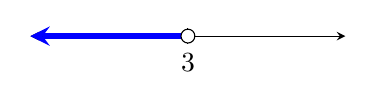
\begin{tikzpicture}
    \draw [<->, >=stealth] (-2,0) -- (2,0);
    \draw (0,0.1) -- (0,-0.1);
    \node at (0,-0.1) [anchor=north] {3};
    \draw [->, >=stealth, line width = 2, color = blue] (0,0) -- (-2,0);
    \draw [fill=white] (0,0) circle (2.5pt);
    \end{tikzpicture}
    &
    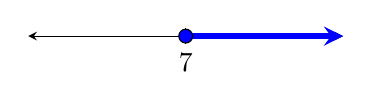
\begin{tikzpicture}
    \draw [<->, >=stealth] (-2,0) -- (2,0);
    \draw (0,0.1) -- (0,-0.1);
    \node at (0,-0.1) [anchor=north] {7};
    \draw [->, >=stealth, line width = 2, color = blue] (0,0) -- (2,0);
    \draw [fill=blue] (0,0) circle (2.5pt);
    \end{tikzpicture}
    &
    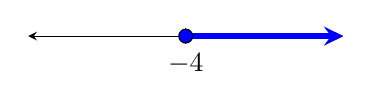
\begin{tikzpicture}
    \draw [<->, >=stealth] (-2,0) -- (2,0);
    \draw (0,0.1) -- (0,-0.1);
    \node at (0,-0.1) [anchor=north] {$-4$};
    \draw [->, >=stealth, line width = 2, color = blue] (0,0) -- (2,0);
    \draw [fill=blue] (0,0) circle (2.5pt);
    \end{tikzpicture} 
    \\[11pt]
13. $x > 0$     &   14. $x \leq -\frac{2}{5}$   &   15. $x < 1$ \\[11pt]
    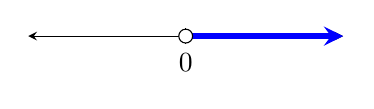
\begin{tikzpicture}
    \draw [<->, >=stealth] (-2,0) -- (2,0);
    \draw (0,0.1) -- (0,-0.1);
    \node at (0,-0.1) [anchor=north] {$0$};
    \draw [->, >=stealth, line width = 2, color = blue] (0,0) -- (2,0);
    \draw [fill=white] (0,0) circle (2.5pt);
    \end{tikzpicture} 
    &
    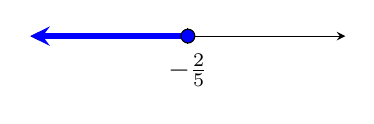
\begin{tikzpicture}
    \draw [<->, >=stealth] (-2,0) -- (2,0);
    \draw (0,0.1) -- (0,-0.1);
    \node at (0,-0.1) [anchor=north] {$-\frac{2}{5}$};
    \draw [->, >=stealth, line width = 2, color = blue] (0,0) -- (-2,0);
    \draw [fill=blue] (0,0) circle (2.5pt);
    \end{tikzpicture}
    &
    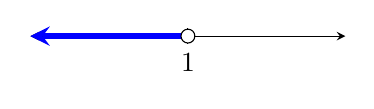
\begin{tikzpicture}
    \draw [<->, >=stealth] (-2,0) -- (2,0);
    \draw (0,0.1) -- (0,-0.1);
    \node at (0,-0.1) [anchor=north] {$1$};
    \draw [->, >=stealth, line width = 2, color = blue] (0,0) -- (-2,0);
    \draw [fill=white] (0,0) circle (2.5pt);
    \end{tikzpicture}
    \\[11pt]
16. All Real Numbers ($\mathbb{R}$) &   17. No Solution ($\varnothing$)    &   18. $x < -6$    \\[11pt]
    
\begin{tikzpicture}
    \draw [<->, >=stealth] (-2,0) -- (2,0);
    \draw (0,0.1) -- (0,-0.1);
    %\node at (0,-0.1) [anchor=north] {$1$};
    \draw [<->, >=stealth, line width = 2, color = blue] (2,0) -- (-2,0);
    %\draw [fill=white] (0,0) circle (2pt);
    \end{tikzpicture}    
    &
    \begin{tikzpicture}
    \draw [<->, >=stealth] (-2,0) -- (2,0);
    \draw (0,0.1) -- (0,-0.1);
    %\node at (0,-0.1) [anchor=north] {$1$};
    %\draw [<->, >=stealth, line width = 2, color = blue] (2,0) -- (-2,0);
    %\draw [fill=white] (0,0) circle (2pt);
    \end{tikzpicture}    
    &
    \raisebox{-0.5cm}{
    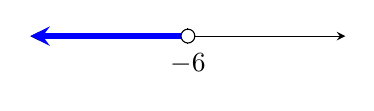
\begin{tikzpicture}
    \draw [<->, >=stealth] (-2,0) -- (2,0);
    \draw (0,0.1) -- (0,-0.1);
    \node at (0,-0.1) [anchor=north] {$-6$};
    \draw [->, >=stealth, line width = 2, color = blue] (0,0) -- (-2,0);
    \draw [fill=white] (0,0) circle (2.5pt);
    \end{tikzpicture}}  \\
\end{tabular}

\end{document}
